\section{Introduction}
\label{sec:introduction}

\par The goal of this laboratory assignment was to optimize a given audio amplifier, and doing both the theoretical and simulation analysis. The architecture of the given circuit can be seen in the following picture.

\begin{figure}[H] \centering
	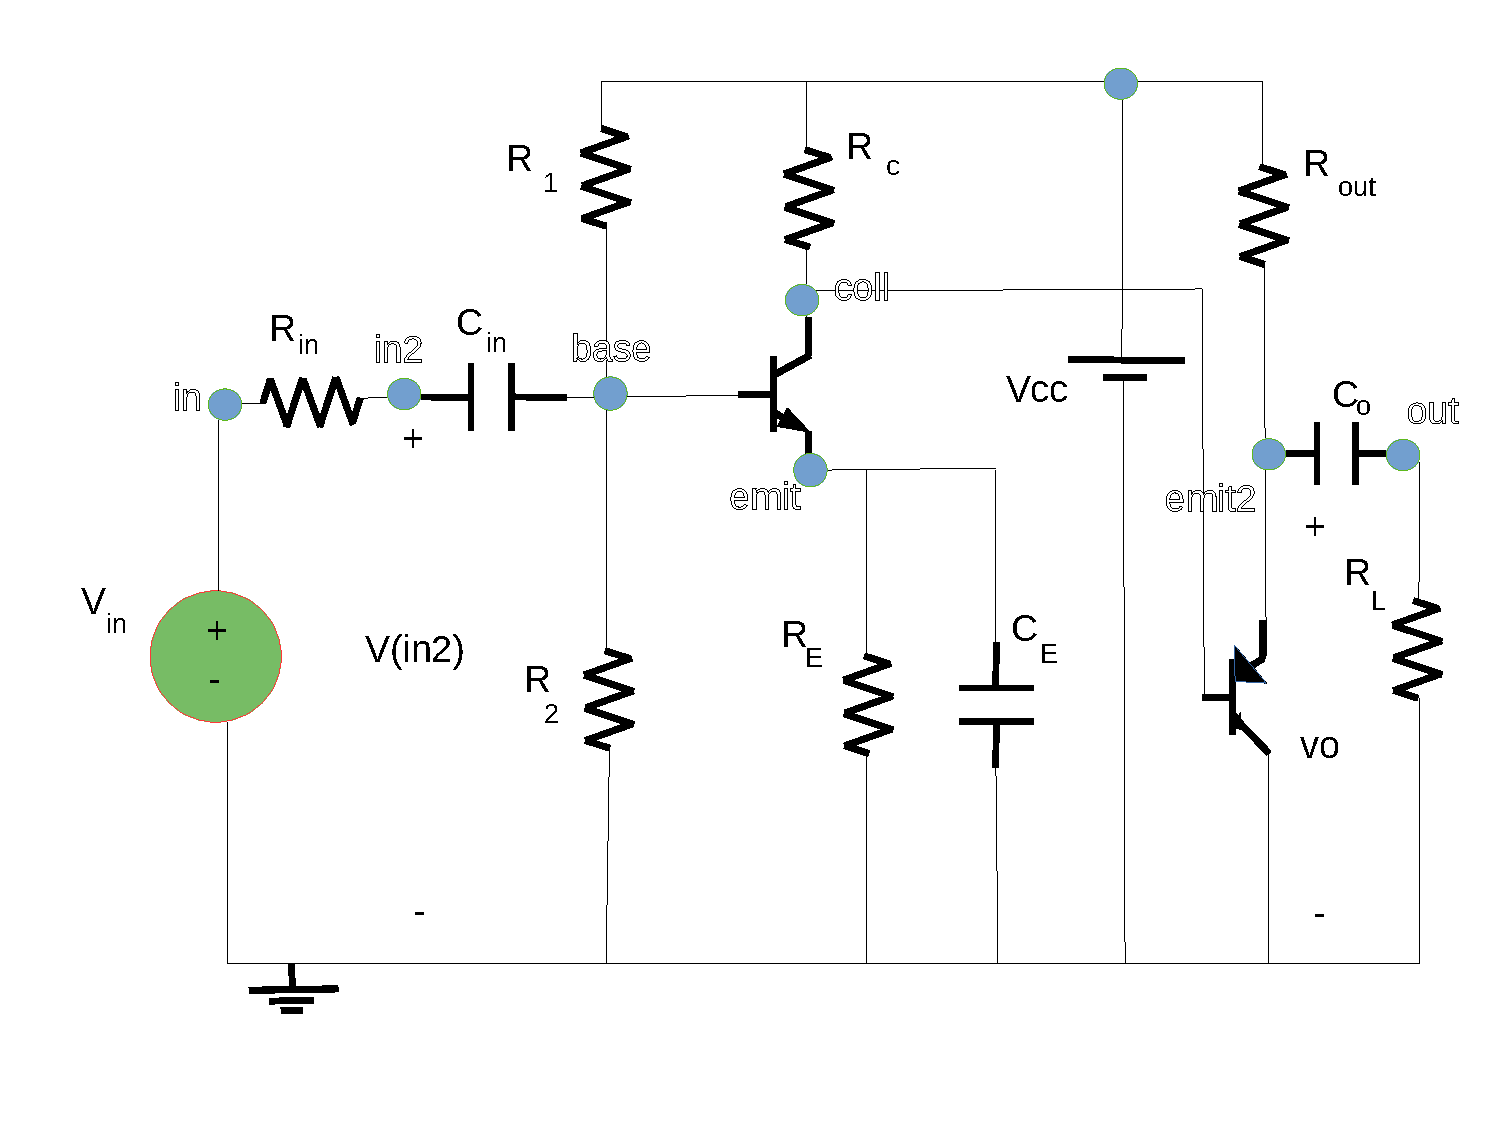
\includegraphics[width=1\linewidth]{lab4.pdf}
	\caption{Audio amplifier - given circuit}
	\label{fig:1}
\end{figure}

\par The input of this circuit is connected to an independent voltage source, which generates an ac signal with an amplitude of $10mV$. The source has an impedance of $100\Omega$, and the amplifier is going to be connected to a speaker which has an impedance of $8\Omega$. As we can see in the previous picture, the circuit is supplied by an independent 12V DC source (vcc).
\par The circuit comprises a gain stage and an output stage, which will be seen in a more detailed way in section \ref{sec:theoretical}. 

\newpage
